\chapter{Introducción}
\label{cap:capitulo1}
\setcounter{page}{1}

\begin{flushright}
\begin{minipage}[]{10cm}
\emph{El éxito es la capacidad de ir de fracaso en fracaso sin perder el entusiasmo.}\\
\end{minipage}\\

Winston Churchill\\
\end{flushright}

\vspace{1cm}


\section{Robótica}
\label{sec:rob}

donde iene este termino
de las esntanforms y primero robot

Los robots se pueden clasificar en dos grupos.
\subsection{Robots de servicio}
Un robot de servicio es un tipo de robot diseñado para realizar tareas en beneficio de los seres humanos. Estos robots están 
destinados a interactuar directamente con las personas y ayudar en diversas actividades. 
Debido a la necesidad de interactuar con los humanos, están equipados con gran variedad de sensores, actuadores y sistemas de 
inteligencia artificial que les permiten percibir y comprender el entorno que los rodea. 
En función de su ámbito de uso, pueden llegar a realizar una amplia gama de tareas, como limpieza y mantenimiento del hogar, 
asistencia en la intervención médica, entrega de alimentos y productos, cuidado de personas mayores, entre otros.

\subsubsection{Robots de campo}
Se considera robot de campo a un robot diseñado para su uso en exterior, bajo unas duras condiciones. Se trata de un sector hetereogenio en el cual se engloban los 
robots espaciales, agrícolas, búsqueda y rescate, inspección de instalaciones, minería, submarinos y conducción autónoma.
\begin{figure} [h!]
  \centering    
  \subfigure[NASA Opportunity]{\label{fig:opportunity}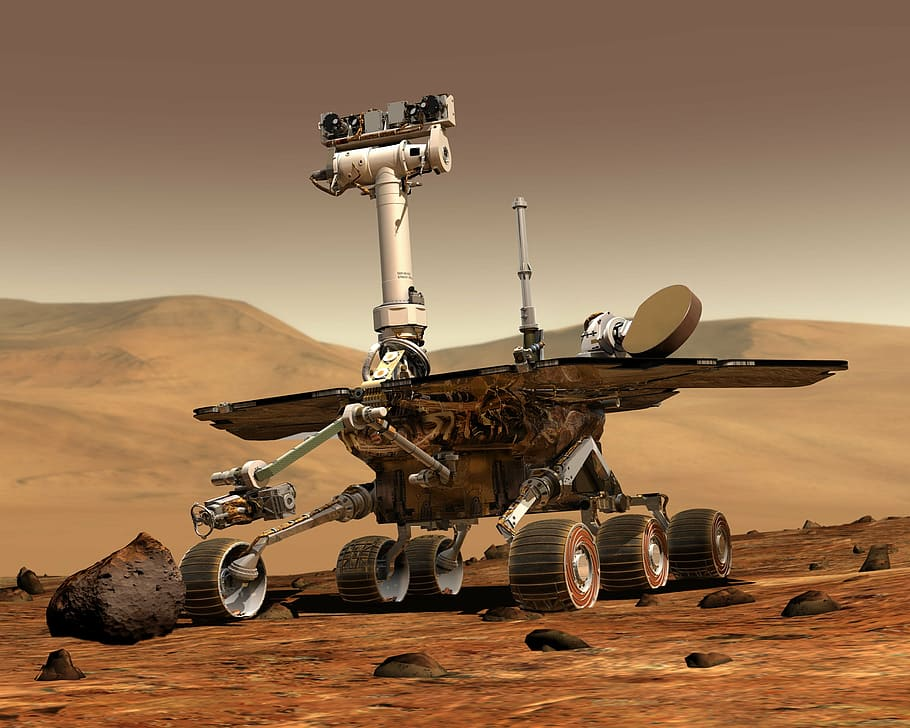
\includegraphics[width=0.3\linewidth ]{figs/rover.jpg}}
  \hspace{3cm}
  \subfigure[Tractor autónomo]{\label{fig:roomba_agua}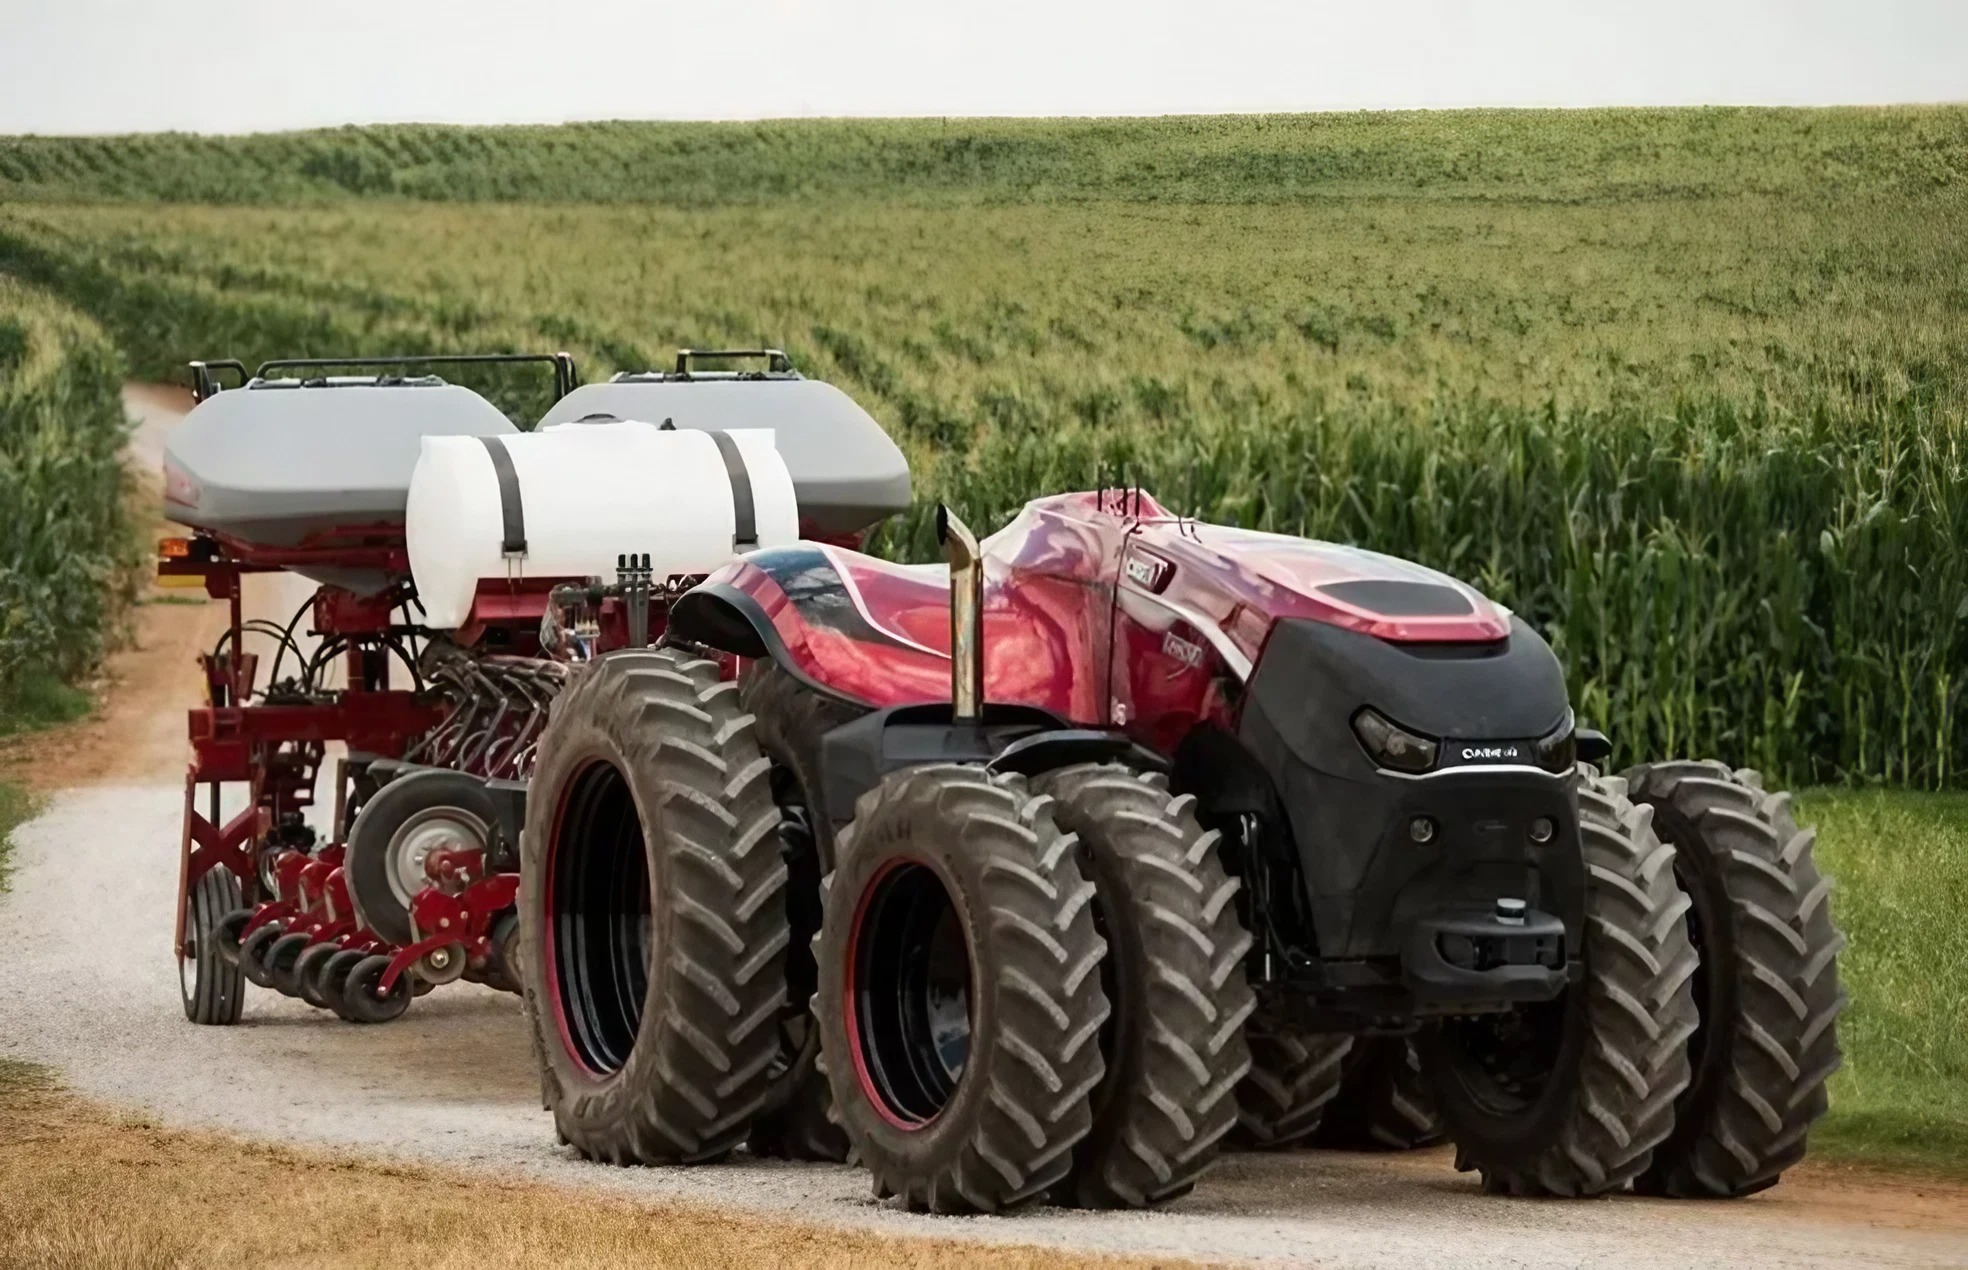
\includegraphics[width=0.3\linewidth]{figs/tractor.jpg}}
  \hspace{3cm}
  \subfigure[Drone de rescate]{\label{fig:drone}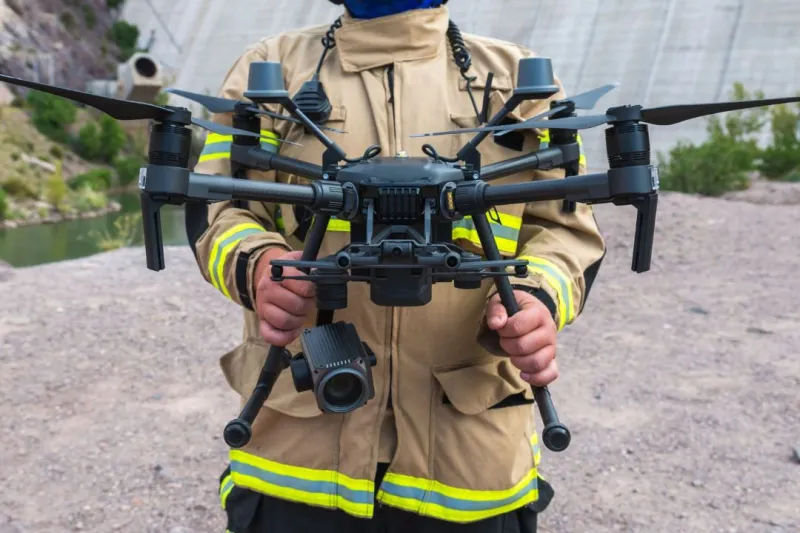
\includegraphics[width=0.3\linewidth]{figs/drone.jpg}}
  \hspace{3cm}
  \subfigure[ROV Victor 6000]{\label{fig:rov}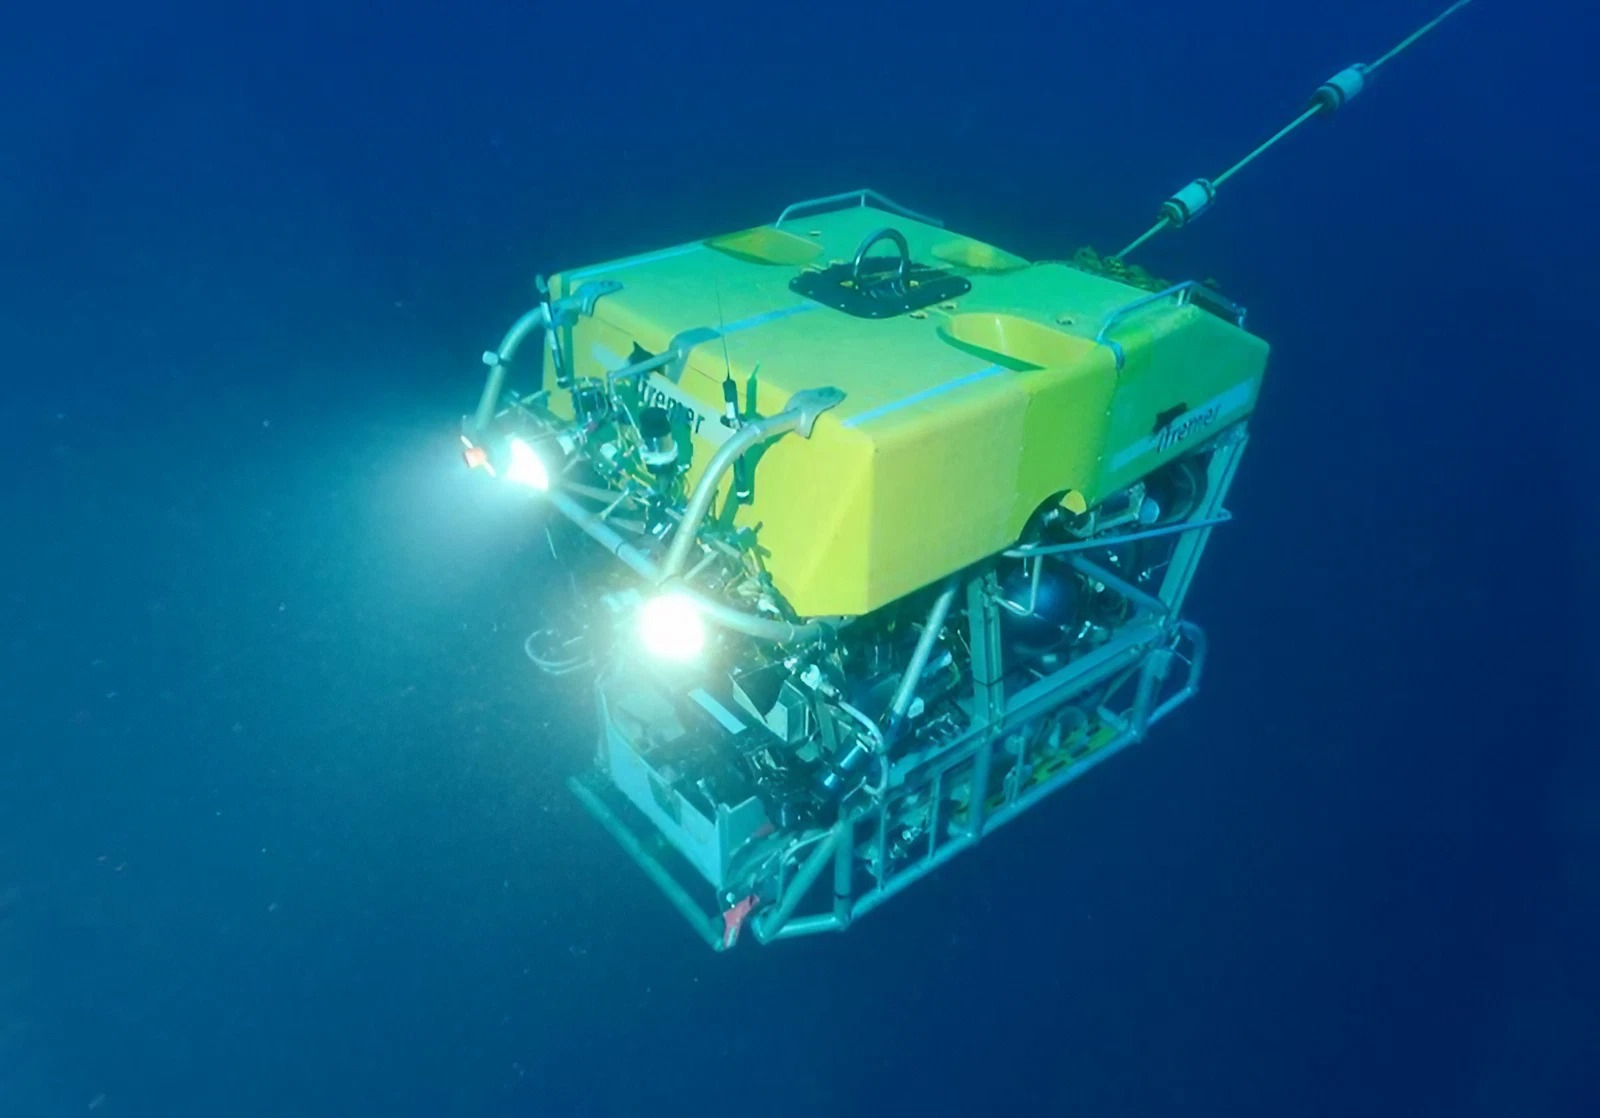
\includegraphics[width=0.3\linewidth]{figs/rov.jpg}}
  \caption{Robots de limpieza}
\end{figure}

\subsubsection{Robots de limpieza}
Son aquellos robots creados para eliminar la suciedad en hogares y empresas. En función de sus características, pueden ser usados para aspirar y fregar el suelo, o incluso,
para limpiar los cristales exteriores de los edificios. Se trata de una tecnología asentada y robusta que a día de hoy cuenta con más de 20 años en el mercado. Pese a esto, 
se pueden encontrar diferentes categorías de robot en función de las necesidades. En la actualidad, integran cada vez más sensores para realizar una limpieza más eficaz y 
en entornos más imprevisibles (cables, animales, objetos tirados, etc).

\begin{figure} [h!]
  \centering    
  \subfigure[Roomba J7+]{\label{fig:roomba}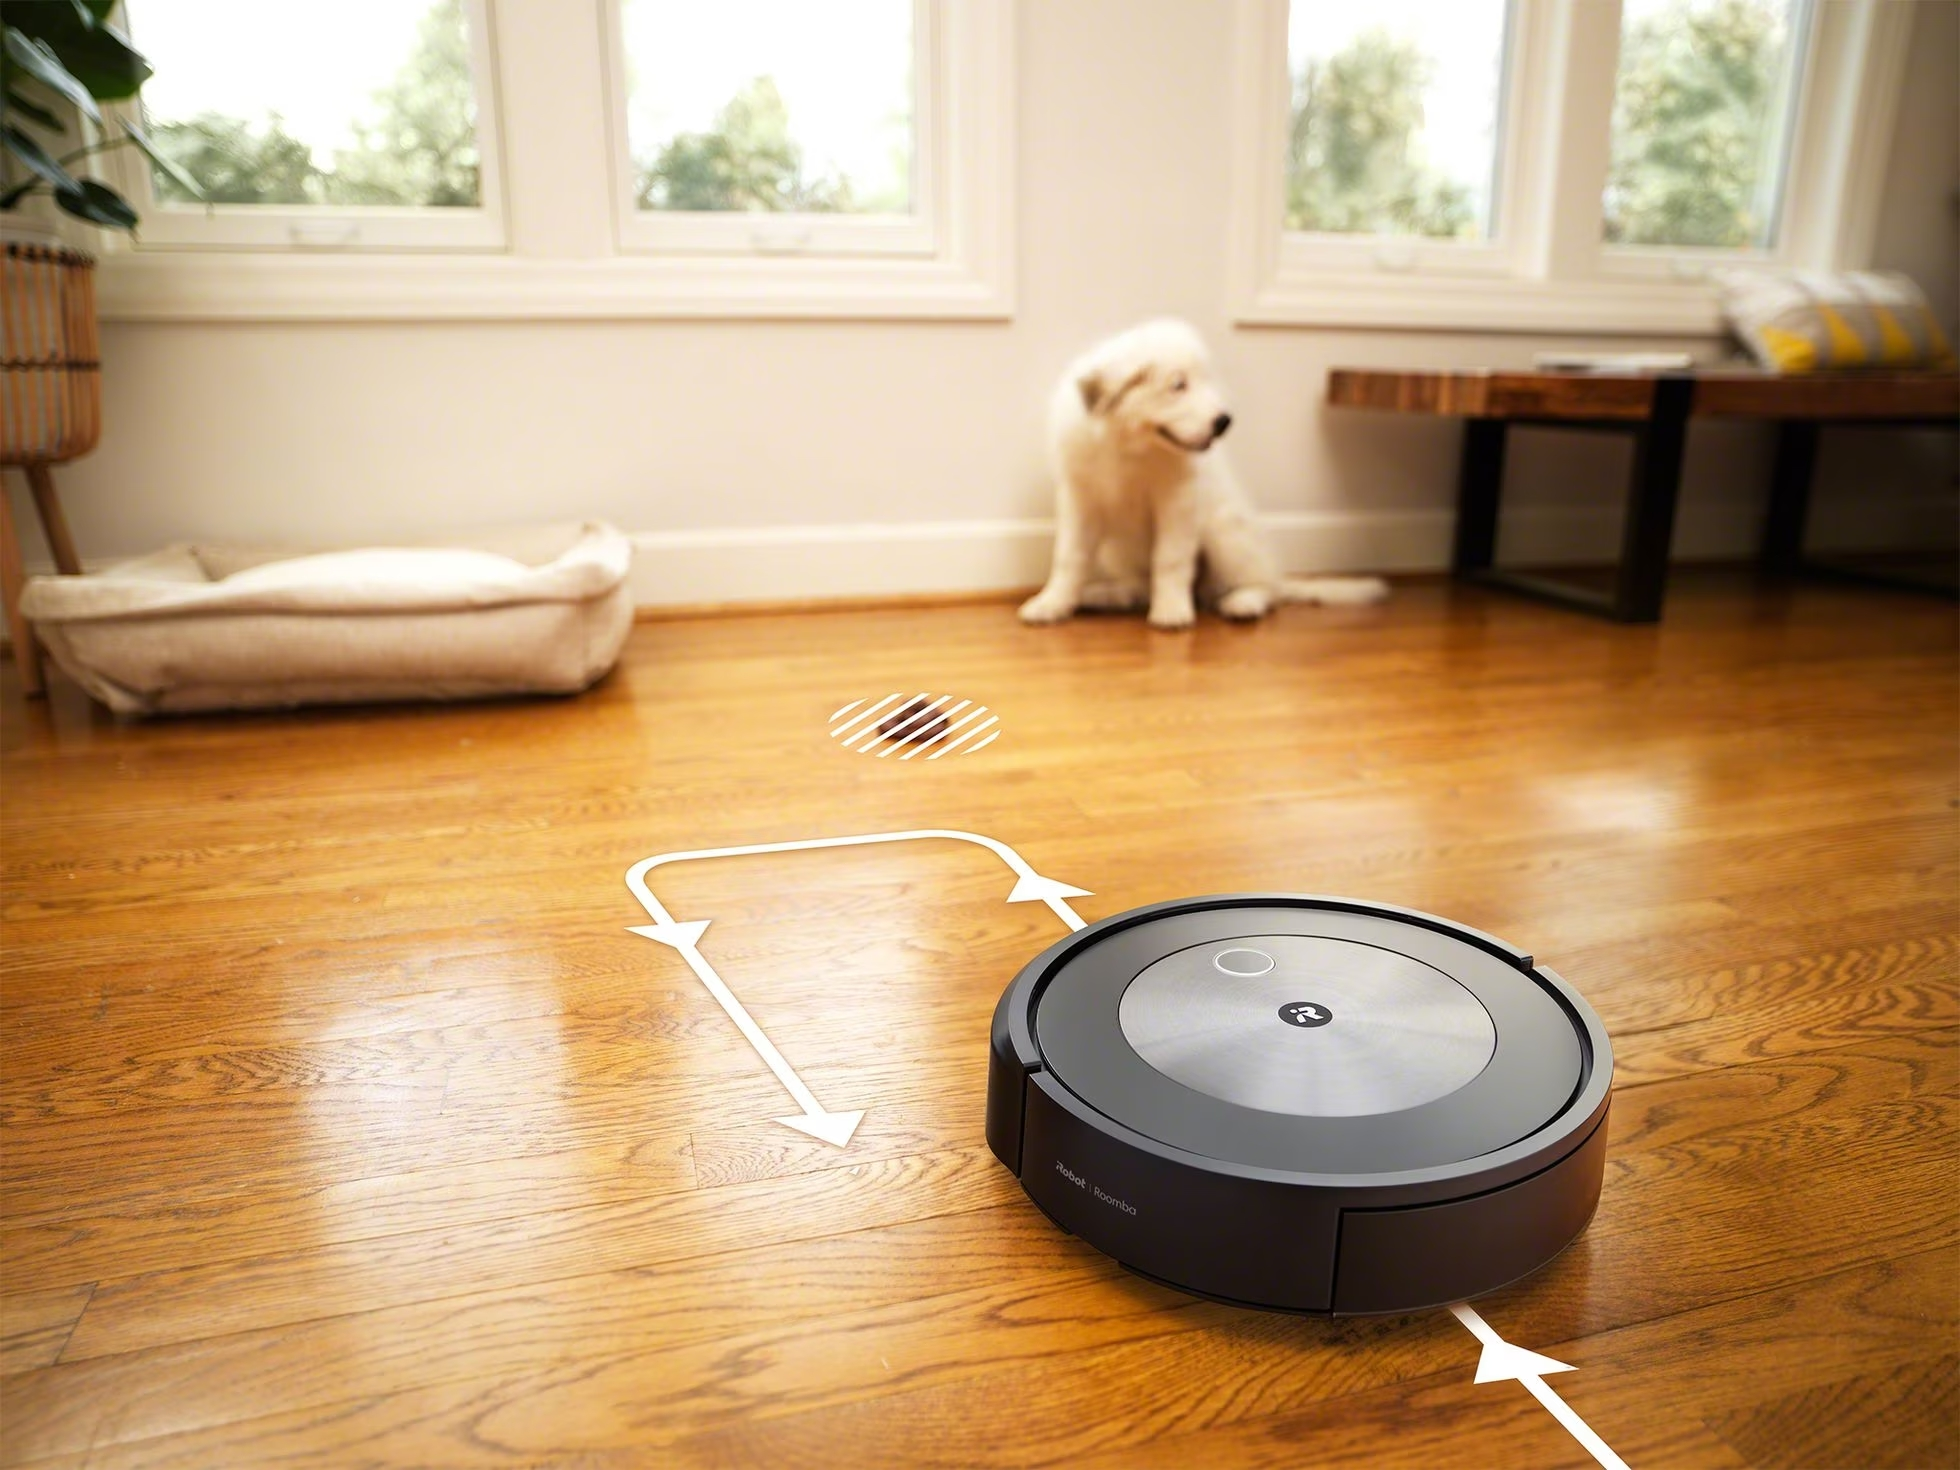
\includegraphics[width=0.3\linewidth ]{figs/roomba.jpg}}
  \hspace{3cm}
  \subfigure[Roomba Braava M6]{\label{fig:roomba_agua}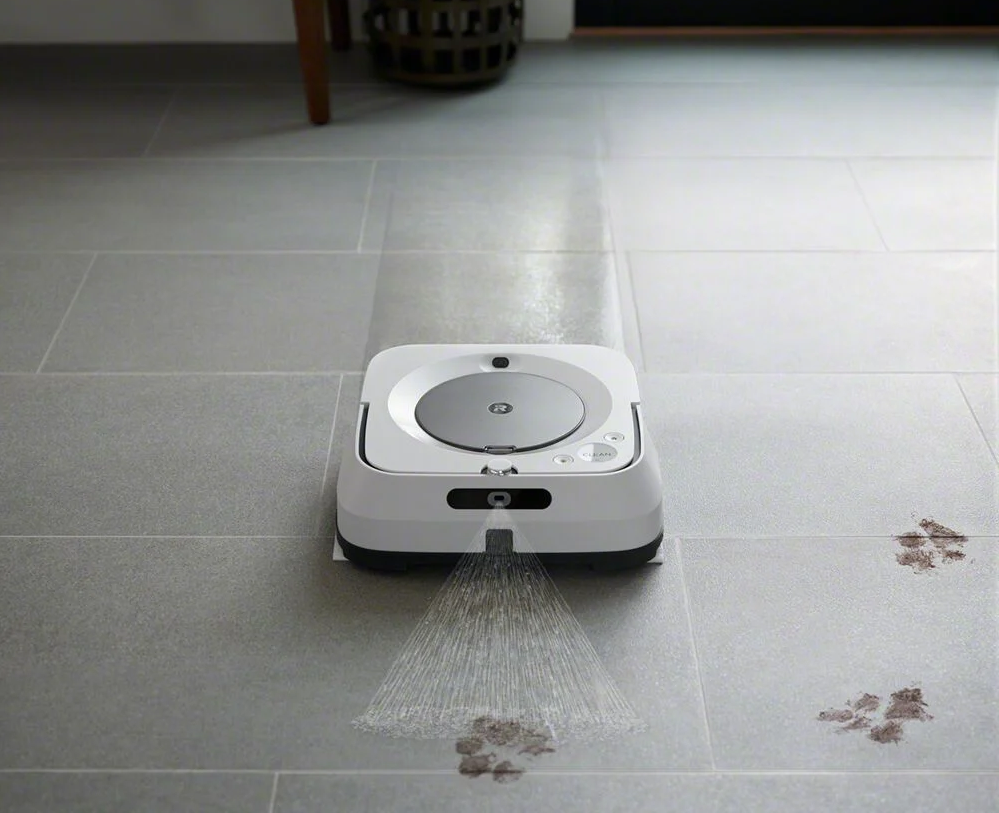
\includegraphics[width=0.3\linewidth]{figs/roombaAgua.jpg}}
  \hspace{3cm}
  \subfigure[Hobot 388]{\label{fig:hobot}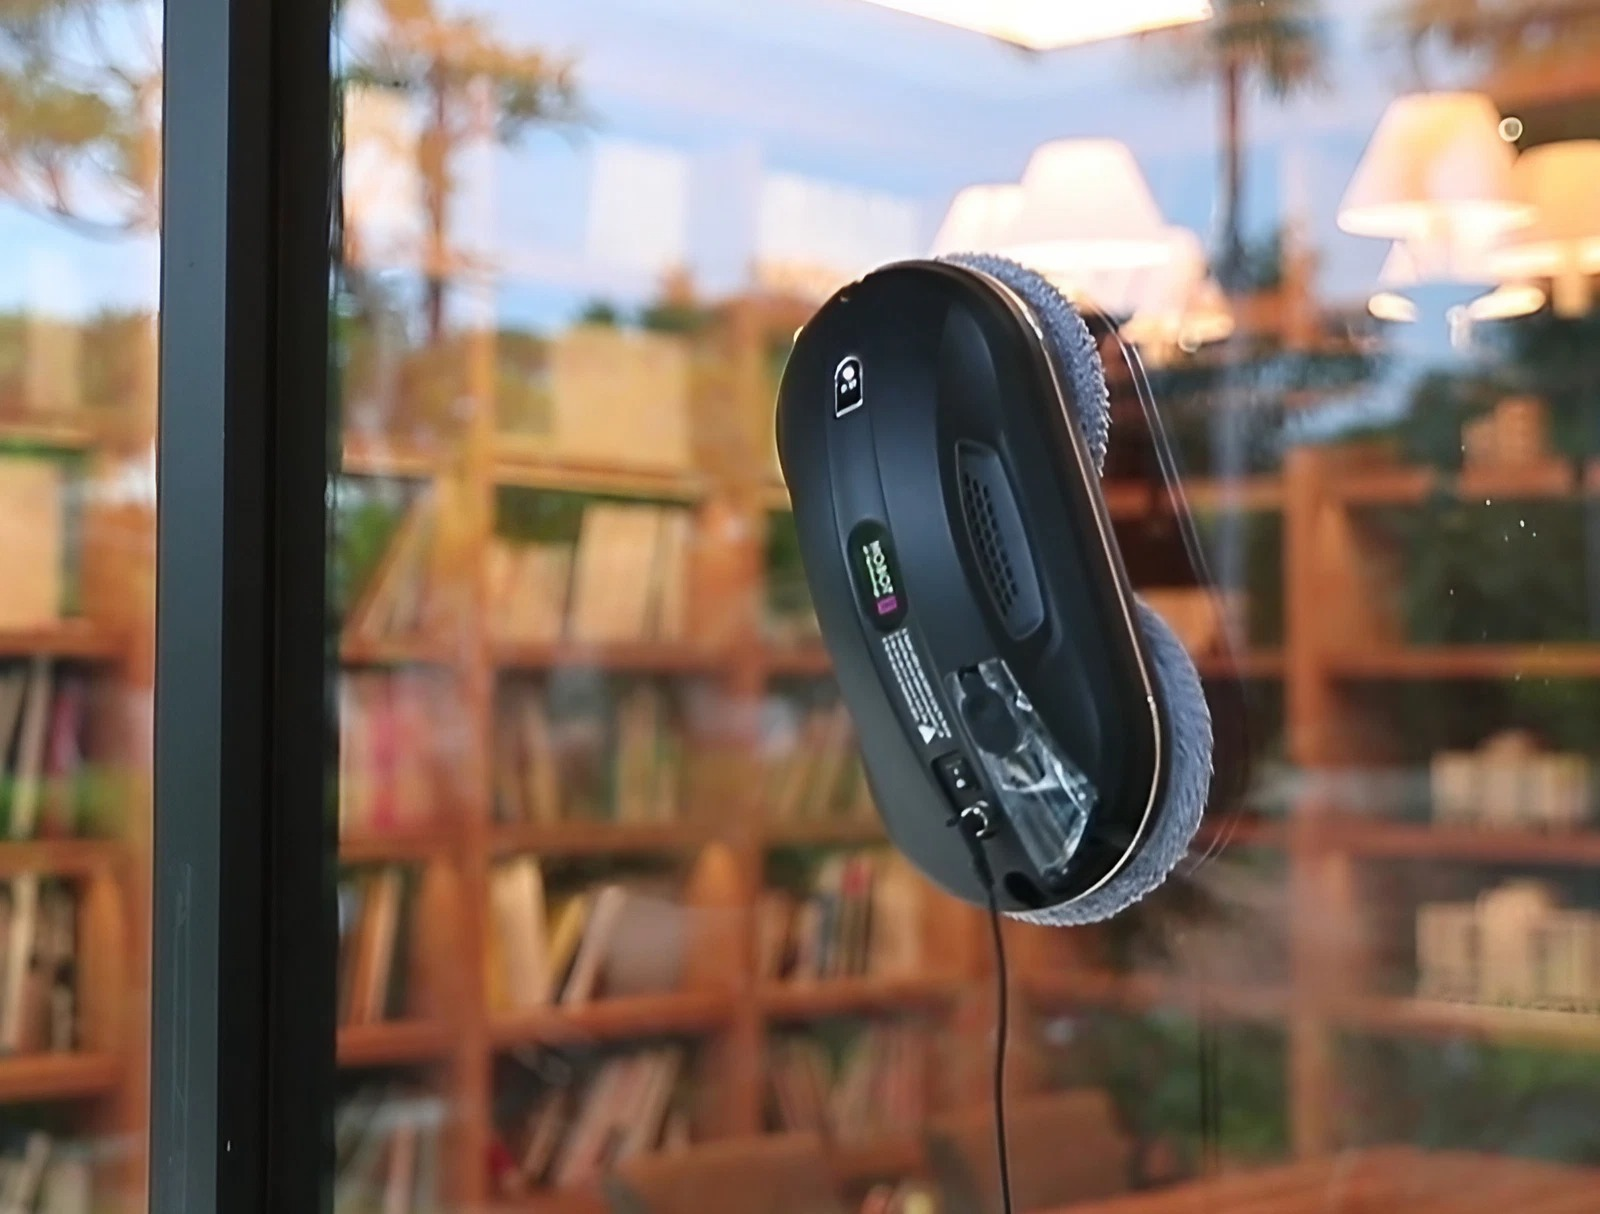
\includegraphics[width=0.3\linewidth]{figs/hobot.jpg}}
  \caption{Robots de limpieza}
\end{figure}



\subsubsection{Robots de entretenimiento}
\subsubsection{Robots en salud}

\subsubsection{Robots en logística}
Los robots de logística están enfocados a tareas de trasporte y organización de mercancías en almacenes y centros de distribución. 
Son capaces de moverse de manera autónoma, cargar y descargar objetos ágilmente y bajo demanda optimizando los procesos logísticos. 
\\Los robots de logística destinados a usarse en almacenes pueden ser clasificados en 2 categorías:
\begin{itemize}
\item \ac{AGV}: Son robots filoguiados, es decir, solo se pueden desplazar a lo largo de un carril preestablecido. Este carril puede ser 
una línea pintada en el suelo o un riel metálico. Son baratos pero son poco flexibles.
\item \ac{AMR}: Son la evolución de los \acs{AGV}. Están dotados con una gran variedad de sensores para poder auto-localizarse y 
detectar obstáculos. Son capaces de navegar autonomamente transportando cargas pesadas, como \textit{palets} o estanterías, en colaboración 
con el resto de la flota. Además son adaptables y fáciles de desplegar pero su coste es más elevado.
\end{itemize}

\begin{figure} [h!]
    \centering    
    \subfigure[Robot AGV Linde C-MATIC \footnote{\url{https://www.linde-mh.es/es/Productos/Carretillas-automatizadas/C-MATIC/}}]{\label{fig:agv}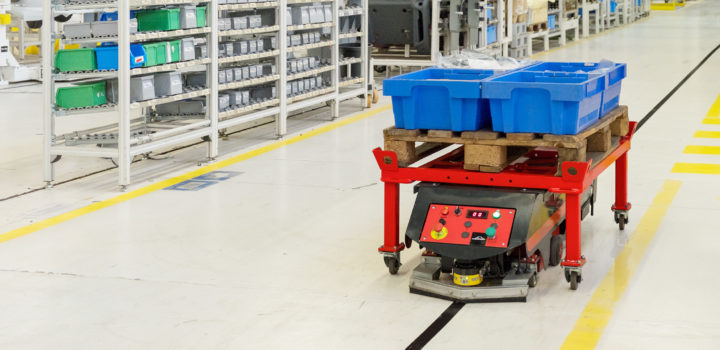
\includegraphics[width=0.4\linewidth ]{figs/agv.jpg}}
    \hspace{1cm}
    \subfigure[Robot AMR Amazon Robotics]{\label{fig:amr}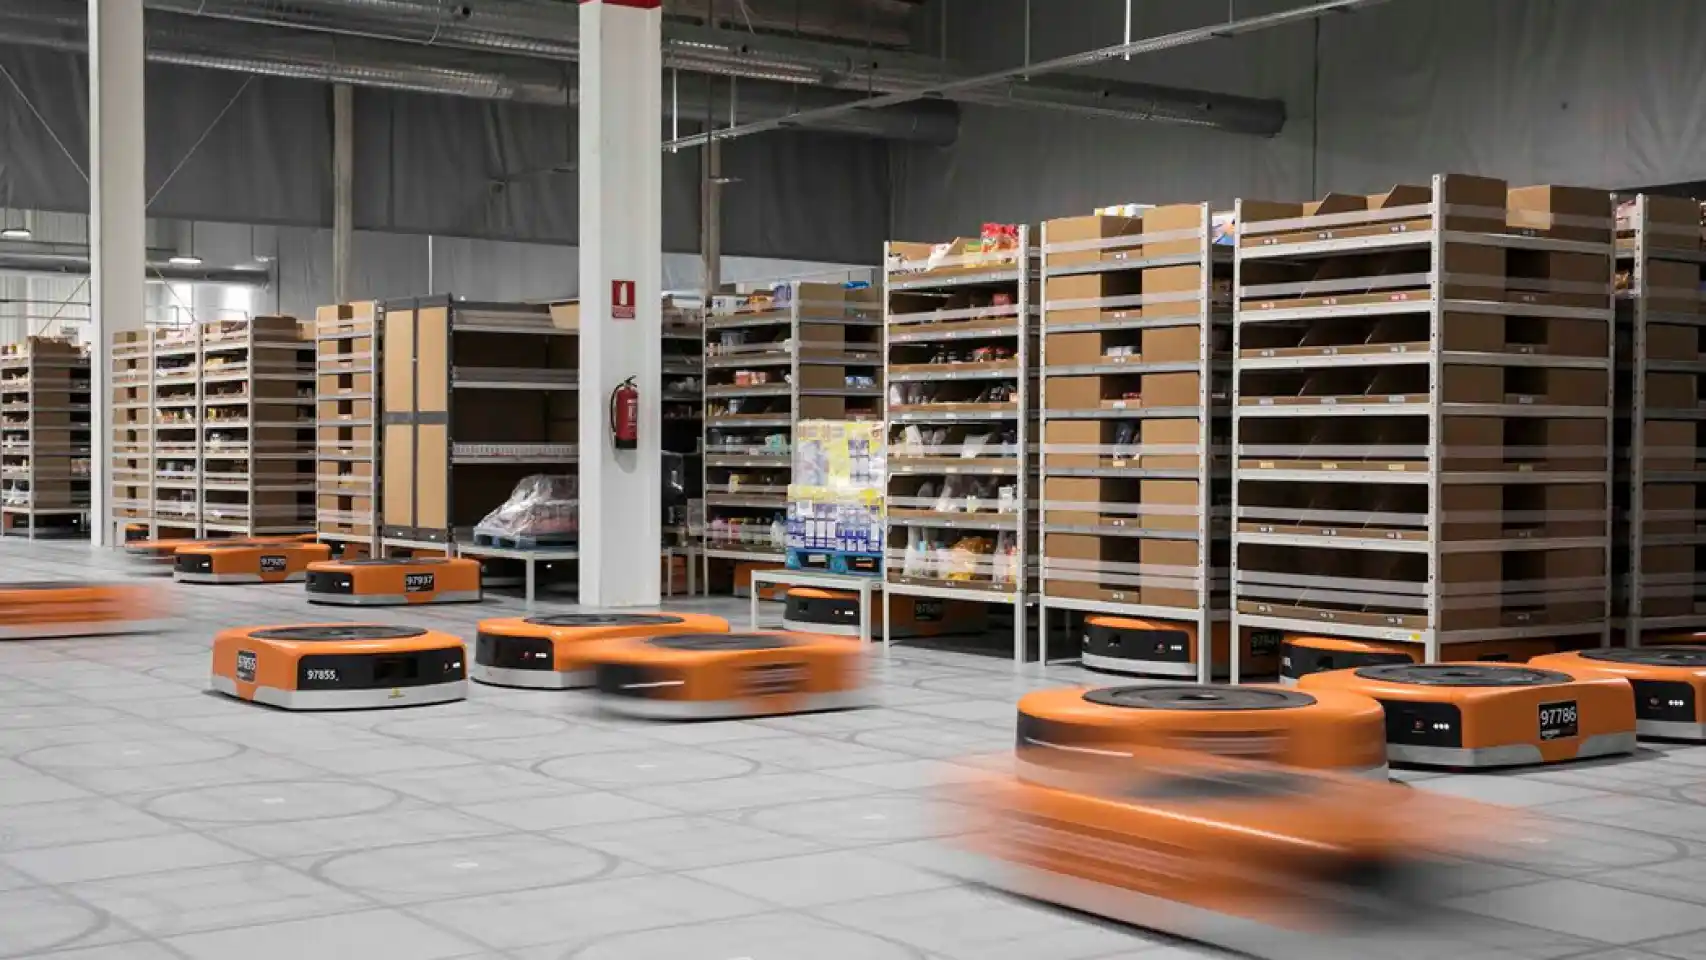
\includegraphics[width=0.4\linewidth]{figs/amr.jpg}}
    \caption{Robots de logística usados en almacenes}
\end{figure}
\newpage
Más allá de su uso de almacenes, cabe destacar los llamados robots de "última milla". Son aquellos usados en el reparto de comida y 
paquetes en las ciudades. Aunque actualmente se encuentra en fase de desarrollo, ya ha sido probados algunos 
prototipos como el usado por Glovo en Londres para repartir comida.
\begin{figure} [ht!]
    \begin{center}
      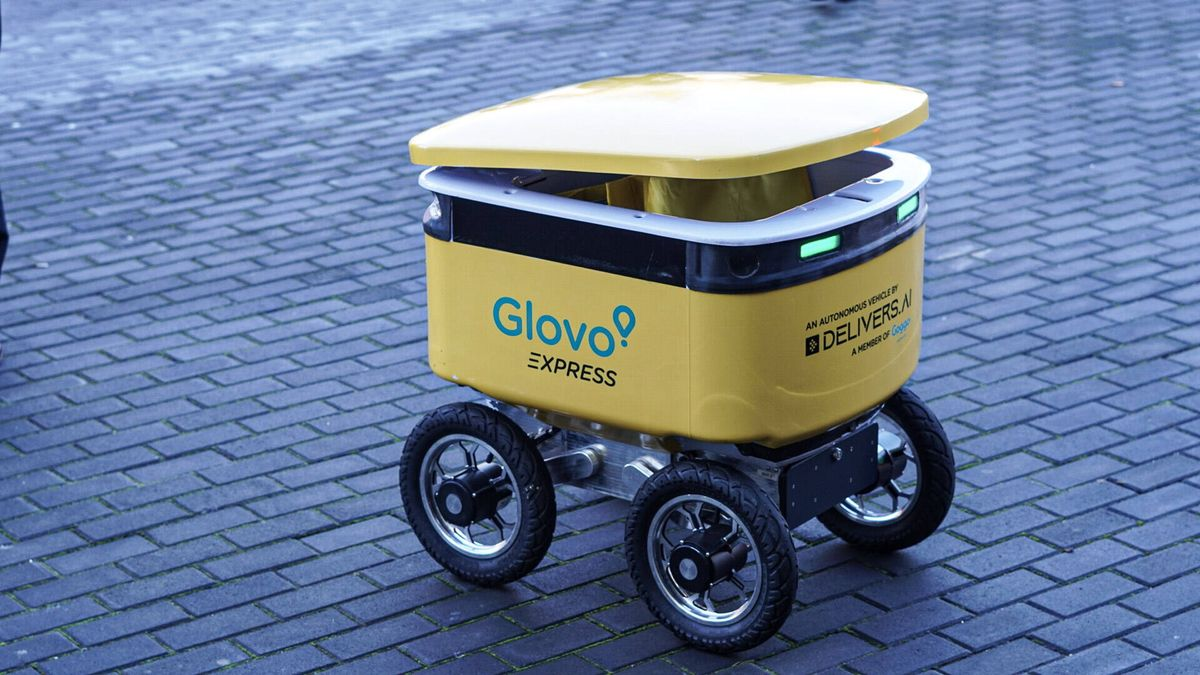
\includegraphics[width=8cm]{figs/reparto.jpg}
    \end{center}
    \caption{Robot de reparto de Glovo}
    \label{fig:glovo}
\end{figure}\ 



\newpage

\subsection{Robots industriales}
Se entiende por robot industrial a una máquina automatizada diseñada específicamente para llevar a cabo tareas en entornos industriales. 
Disponen de numerosas articulaciones y una gran capacidad de maniobrabilidad. Su objetivo principal es remplazar a un 
operario humano en tareas aburridas, sucias, peligrosas y exigentes (\textit{4D: Dull, Dirty, Dangerous and Demanding}).

\section{Robótica industrial}
\label{sec:rob_industrial}


\subsection{SCARA}
\subsection{Articulados}
\subsection{Paralelos}
\subsection{Cartesianos}

\section{Robótica educativa}
\label{sec:rob_educativa}
\subsection{Robótica en institutos}
\subsection{Robótica en universidades}

\section{Robótica de bajo coste}
\label{sec:rob_bajo:coste}

